\section{Curvature bounds and the injectivity condition}\label{sec:injectivity}

Baek proves the injectivity condition for a balanced maximum cap $K$ with rotation angle $\pi/2$ from the
inequality $\sigma_K\le k_0(g_K^+(t))\dd t$ on $[0,\pi/2)$ \baek{Thm.~6.4.3}, which is the limit of
$\sigma_{K_n}(t)\le k_0(g_{K_n}^+(t))\delta+O(\delta^2)$ for maximum polygon caps $K_n$ with step size
$\delta$ \baek{Thm.~6.3.3}; the proof of the latter uses the balance $\sigma=\tau$. For the polygon caps of
\cref{sec:selection} the defect bound of \cref{prop:floating} replaces the balance, and its errors add up to at most $2\eta$
by \eqref{eq:weights}. In this section we use \cref{sec:selection,sec:variations} with $\omega=\pi/2$ and $\cA=\cA_{\pi/2}$: $K_*\in\Kc_{\pi/2}$ is a maximizing cap with
$\cA(K_*)>0$, $\Theta_k=\{j\delta:0<j<n\}$ with $n=2^{k+1}$ and step size $\delta=\delta_k=\pi/(2n)\le\pi/4$. All the normals of $\Theta_k$ are floating.
A polygon cap $K\in\Kc_k$ has no edge with normal angle $0$ or $\pi$ and none with normal in $(-\pi/2,0)$; its
edge normals are among $\delta,2\delta,\dots,(2n-1)\delta$ and $3\pi/2$. For an angle $u$ let
$H^{\mathrm b}_K(u)$ and $H^{\mathrm d}_K(u)$ be as in \cref{sec:Q}, so that $Q^-_K(u)$ is the complement of
$H^{\mathrm b}_K(u)\cup H^{\mathrm d}_K(u)$.

\subsection{One normal of a polygon cap}

\begin{lemma}[the inner wall near the corner]\label{lem:wall}
Let $K\in\Kc_k$, $t\in\Theta_k$, $q=\tan(\delta/2)$, and $\xx=\xx_K(t)$. Let $\vec b=\vec b_K(t)=\{\xx-sv_t:s\ge0\}$.
Then the set of $s\ge0$ with $\xx-sv_t\in H^{\mathrm d}_K(t-\delta)$ is $[0,\alpha_-]$ and the set of $s\ge0$ with
$\xx-sv_t\in H^{\mathrm d}_K(t+\delta)$ is $[0,\alpha_+]$, where
\[
  \alpha_-=\tan\delta\,\bigl(g_K^-(t)-1+q\bigr),\qquad\alpha_+=\tan\delta\,\bigl(1-g_K^+(t)+q\bigr)
\]
(an interval is empty if its right end is negative); and the set of $s\in\R$ with
$\xx-sv_t\in H^{\mathrm b}_K(t-\delta)\cap H^{\mathrm b}_K(t+\delta)$ is an interval, empty or of length $2q-\sigma_K(t)$.
\end{lemma}

This is \baek{Lemma~6.3.2}, together with the length $2\tan(\delta/2)-\sigma_K(t)$ that Baek asserts in the proof of \baek{Thm.~6.3.3}. They are stated there for maximum polygon
caps, but the proofs use only that no normal angle of $K$ lies in $(t-\delta,t)\cup(t,t+\delta)\cup(t+\frac\pi2-\delta,t+\frac\pi2)\cup(t+\frac\pi2,t+\frac\pi2+\delta)$, which holds for
every $K\in\Kc_k$.

\begin{proof}
Since no normal angle of $K$ lies between $t+\pi/2$ and $t+\delta+\pi/2$, the supporting lines $l_K(t+\pi/2)$ and
$l_K(t+\delta+\pi/2)$ meet at a vertex $r$ of $K$, namely $r=C_K^+(t)=\yy_K(t)-g_K^+(t)u_t$, and
$h_K(t+\delta+\pi/2)=\ip r{v_{t+\delta}}$. As $\xx-r=(g_K^+(t)-1)u_t-v_t$,
\begin{align*}
  \ip{\xx}{v_{t+\delta}}-h_K(t+\delta+\tfrac\pi2)+1&=\ip{\xx-r}{v_{t+\delta}}+1\\
  &=-(g_K^+(t)-1)\sin\delta-\cos\delta+1 .
\end{align*}
Now $\ip{\xx-sv_t}{v_{t+\delta}}=\ip{\xx}{v_{t+\delta}}-s\cos\delta$, so $\xx-sv_t\in H^{\mathrm d}_K(t+\delta)$ iff
$s\le\alpha_+=\bigl[(1-g_K^+(t))\sin\delta+1-\cos\delta\bigr]/\cos\delta$, and $(1-\cos\delta)/\cos\delta=\tan\delta\tan(\delta/2)$. For $t-\delta$
use $r'=C_K^-(t)=\yy_K(t)-g_K^-(t)u_t$ in the same way. Next, $\ip{\xx-sv_t}{u_{t\mp\delta}}=\ip\xx{u_{t\mp\delta}}\pm s\sin\delta$, so the
conditions $\ip p{u_{t-\delta}}\ge h_K(t-\delta)-1$ and $\ip p{u_{t+\delta}}\ge h_K(t+\delta)-1$ on
$p=\xx-sv_t$ read $s\ge s_-$ and $s\le s_+$ with
\begin{align*}
  s_+-s_-&=\frac{2\cos\delta\,(h_K(t)-1)-h_K(t+\delta)-h_K(t-\delta)+2}{\sin\delta}\\
  &=\frac{2(1-\cos\delta)-\sigma_K(t)\sin\delta}{\sin\delta}=2q-\sigma_K(t),
\end{align*}
where we used $u_{t+\delta}+u_{t-\delta}=2\cos\delta\,u_t$, $\ip\xx{u_t}=h_K(t)-1$ and, since no normal angle of $K$ lies in $(t-\delta,t)\cup(t,t+\delta)$,
$h_K(t+\delta)+h_K(t-\delta)-2\cos\delta\,h_K(t)=\sigma_K(t)\sin\delta$ (equality in the
inequality in the proof of \cref{lem:usc}).
\end{proof}

\begin{lemma}[the polygon bound at one normal]\label{lem:tau}
For $K\in\Kc_k$ and $t\in\Theta_k$,
\begin{multline*}
  \tau_K(t)\le\max\Bigl(\tan\delta\,(g_K^-(t)-1+q),\ \tan\delta\,(1-g_K^+(t)+q),\ 0\Bigr)\\
  +\max\bigl(2q-\sigma_K(t),0\bigr),\qquad q=\tan\tfrac\delta2 .
\end{multline*}
\end{lemma}

\begin{proof}
Let $X=\partial\cN_{\Theta_k}(K)\cap\vec b_K(t)$; by \cref{fact:sides}\ref{fact:sides:wall}, $\tau_K(t)=\Hone(X)$. As
$X\subset\clos\cN_{\Theta_k}(K)\subset\{y\ge0\}$ and the
line $b_K(t)$ is not horizontal, at most one point of $X$ lies on the $x$-axis. Let $p\in X$ with
$p_y>0$. The set $\cN_{\Theta_k}(K)$ is open in $\{y\ge0\}$, being a union of open quarter-planes
intersected with that half-plane; so the boundary point $p$ is not in it, and $p\notin Q^-_K(u)$ for
every $u\in\Theta_k$. Also $Q^-_K(0)$ and $Q^-_K(\pi/2)$ lie in $\{y<0\}$ (the inner corners $\xx_K(0)$ and
$\xx_K(\pi/2)$ are on the $x$-axis). As $t-\delta,t,t+\delta\in\Theta_k\cup\{0,\pi/2\}$, $p\notin Q^-_K(u)$ for
$u\in I=\{t-\delta,t,t+\delta\}$; so either $p\in H^{\mathrm d}_K(u)$ for some $u\in I$, or $p\in H^{\mathrm b}_K(u)$ for all $u\in I$.
On $\vec b_K(t)$, $H^{\mathrm d}_K(t)$ contains only the corner $\xx$, and $H^{\mathrm b}_K(t)$ everything. By
\cref{lem:wall}, the points of the first kind form a set of length at most
$\max(0,\alpha_-,\alpha_+)$, those of the second kind a set of length at most $\max(0,2q-\sigma_K(t))$.
\end{proof}

\begin{figure}[ht]
\centering
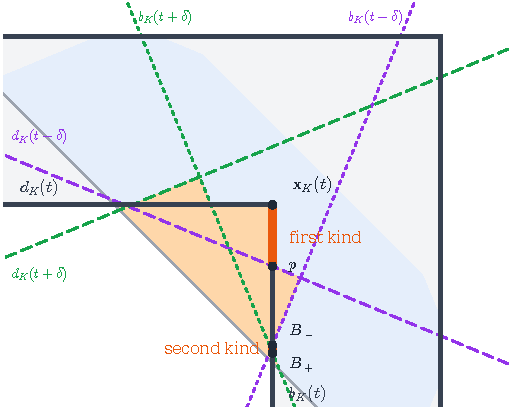
\includegraphics[width=0.8\linewidth]{figures/fig-wall}
\caption{\cref{lem:wall,lem:tau}, for the polygon cap with the angle set $\Theta_1$ ($n=4$, $\delta=\pi/8$) and the support values of Gerver's cap, at $t=\pi/4$, drawn in the frame of the supporting hallway $L_K(t)$ (the polygon niche is shaded). The part of $\vec b_K(t)$ above the dashed line $d_K(t-\delta)$ is the segment $[p,\xx_K(t)]$ (points of the first kind); further down $\vec b_K(t)$ runs between the dotted lines $b_K(t-\delta)$ and $b_K(t+\delta)$, from $B_-$ to $B_+$ (points of the second kind). The side of the niche on $\vec b_K(t)$ lies in the union of the two segments.}
\label{fig:wall}
\end{figure}

\begin{lemma}[with a defect]\label{lem:curv-defect}
Let $K\in\Kc_k$, $t\in\Theta_k$, $e\ge0$, $D\ge0$ with $g_K^+(t)\le D$ and $\sigma_K(t)\le\tau_K(t)+e$. Then
\[
  \sigma_K(t)\le k_0\bigl(g_K^+(t)\bigr)\,\delta+(D+4)\delta^2+e .
\]
\end{lemma}

\begin{proof}
Let $M=\abs{g_K^+(t)-1}\le D+1$. As $0\le g_K^-\le g_K^+$, each of $g_K^--1+q$ and $1-g_K^++q$ is at most $M+q$, so the first maximum
in \cref{lem:tau} is at most $\tan\delta\,(M+q)\le\delta M+(D+3)\delta^2$, using $\tan\delta\le\delta+\delta^2$, $q\le\delta$ and
$\delta\le1$. If $\sigma_K(t)\ge2q$, the second maximum is $0$ and
$\sigma_K(t)\le\tau_K(t)+e\le\delta M+(D+3)\delta^2+e$. If $\sigma_K(t)<2q$, then
$\sigma_K(t)\le\delta M+(D+3)\delta^2+(2q-\sigma_K(t))+e$ and $2q\le\delta+\delta^2$, so
$\sigma_K(t)\le\frac{M+1}2\delta+\frac{D+4}2\delta^2+\frac e2$. Both $M$ and $(M+1)/2$ are at most $k_0(g_K^+(t))$.
\end{proof}

\subsection{From normals to intervals}

\begin{lemma}[arms between two steps]\label{lem:cell}
Let $K\in\Kc_k$ have diameter at most $D$, and let $t\in\{0\}\cup\Theta_k$. Then $g_K^+$ is nonincreasing on
$[t,t+\delta)$, and $g_K^+(t)-g_K^+(u)\le D\delta$ for $u\in(t,t+\delta)$.
\end{lemma}

This is \baek{Lemma~6.4.1}, with $D$ in place of the bound $5$ for maximum polygon caps. The half-open interval is needed: $g_K^+$ jumps up at $t+\delta$, by $\sigma_K(t+\delta+\pi/2)$, and Baek's statement compares $g_K^+(t)$ with $g_K^-(t+\delta)$.

\begin{proof}
Since there is no normal angle of $K$ strictly between $t$ and $t+\delta$, nor between $t+\pi/2$ and
$t+\delta+\pi/2$, there are vertices $A$ and $C$ of $K$ with $A_K^\pm(s)=A$ and $C_K^\pm(s)=C$ for
$s\in(t,t+\delta)$, and also $A_K^+(t)=A$, $C_K^+(t)=C$. As $\yy_K(s)$ lies on $l_K(s)\ni A$, we get
$g_K^+(s)=\ip{A-C}{u_s}$ on $[t,t+\delta)$. Its derivative is $\ip{A-C}{v_s}$. It is at most $0$,
because $\ip A{v_s}\le h_K(s+\pi/2)=\ip C{v_s}$, and at least $-\norm{A-C}\ge-D$.
\end{proof}

\begin{lemma}[summing the steps]\label{lem:sum}
Let $K\in\Kc_k$ have diameter at most $D$ with $k_0(g_K^+)\le B$ on $[0,\pi/2]$, and suppose that for some $C\ge0$ and every
$t\in\{0\}\cup\Theta_k$
\[
  \sigma_K(t)\le k_0(g_K^+(t))\,\delta+C\delta^2+e(t),\qquad e(t)\ge0 .
\]
Then for $-\pi/2\le a<b\le\pi/2$ with $a'=\max(a,0)\le b$,
\[
  \sigma_K\bigl((a,b)\bigr)\le\int_{a'}^bk_0\bigl(g_K^+(u)\bigr)\dd u+\Bigl(B+\frac\pi2(C+D)\Bigr)\delta+\sum_{j=0}^{n-1}e(j\delta).
\]
\end{lemma}

\begin{proof}
On $(-\pi/2,\pi/2)$, $\sigma_K$ is carried by the points $j\delta$, $1\le j\le n-1$. For $t=j\delta$,
$0\le j\le n-1$, \cref{lem:cell}, together with $k_0$ being $1$-Lipschitz, gives
$k_0(g_K^+(t))\delta\le\int_t^{t+\delta}k_0(g_K^+)+D\delta^2$, so
$\sigma_K(t)\le\int_t^{t+\delta}k_0(g_K^+)+(C+D)\delta^2+e(t)$. Sum over the grid points $t\in[a',b)$; they
are at most $n$ in number, their cells $[t,t+\delta)$ lie in $[a',b+\delta)$ and the part beyond $b$ is shorter than $\delta$,
where $k_0(g_K^+)\le B$. Also $n(C+D)\delta^2=\frac\pi2(C+D)\delta$.
\end{proof}

The next two lemmas are the passage to the limit in the proof of \baek{Thm.~6.4.3}. Baek gets the lower semicontinuity of the mass of an open interval from the weak convergence of
$\sigma_{K_n}$ and the Portmanteau theorem; Lemma~\ref{lem:lsc} replaces this by a direct argument with support functions.

\begin{lemma}[lower semicontinuity of the mass of an open interval]\label{lem:lsc}
If convex bodies $K_j\to K$ in $\dH$ and $a<b$, then $\sigma_K((a,b))\le\liminf_j\sigma_{K_j}((a,b))$.
\end{lemma}

\begin{proof}
For $0<\eps<\pi$ let $\Phi_K(\eps)=\ip{v_K(b-\eps,b)}{v_b}-\ip{v_K(a,a+\eps)}{v_a}+\int_a^bh_K$. A point
$p=h_K(b)u_b+mv_b$ of $e_K(b)$ lies in $H_K(b-\eps)$, i.e. $h_K(b)\cos\eps-m\sin\eps\le h_K(b-\eps)$, so
$\ip{v_K^-(b)}{v_b}\ge\ip{v_K(b-\eps,b)}{v_b}$; likewise $\ip{v_K^+(a)}{v_a}\le\ip{v_K(a,a+\eps)}{v_a}$. By
\eqref{eq:sigma-open}, $\Phi_K(\eps)\le\sigma_K((a,b))$, and $\Phi_K(\eps)\to\sigma_K((a,b))$ as $\eps\downarrow0$ by
\cref{fact:convex}\ref{fact:convex:vertices}. For fixed $\eps$, $\Phi_{K_j}(\eps)\to\Phi_K(\eps)$, as $\Phi$ is an explicit
continuous function of the support function. Hence
$\sigma_K((a,b))=\lim_\eps\lim_j\Phi_{K_j}(\eps)\le\liminf_j\sigma_{K_j}((a,b))$.
\end{proof}

\begin{lemma}[passing to the limit]\label{lem:limit}
Let $K_j$ be polygon caps with rotation angle $\pi/2$ that converge in $\dH$ to $K\in\Kc_{\pi/2}$, and let $\eps_j\to0$
be such that, for all $-\pi/2\le a<b\le\pi/2$ with $a'=\max(a,0)\le b$,
\[
  \sigma_{K_j}\bigl((a,b)\bigr)\le\int_{a'}^bk_0\bigl(g_{K_j}^+\bigr)+\eps_j .
\]
Then $\sigma_K(E)\le\int_Ek_0(g_K^+(t))\dd t$ for every Borel set $E\subset[0,\pi/2)$.
\end{lemma}

\begin{proof}
By \cref{fact:iteration}\ref{fact:iteration:arms} and since $k_0$ is $1$-Lipschitz,
$\int_{a'}^bk_0(g_{K_j}^+)\to\int_{a'}^bk_0(g_K^+)$. With \cref{lem:lsc},
$\sigma_K((a,b))\le\int_{a'}^bk_0(g_K^+)$ for all such $a<b$. A nonempty relatively open interval of $[0,\pi/2)$ is $(a,b)$ with $a\ge0$, or $[0,b)\subset(a,b)$ for every
$a\in[-\pi/2,0)$, so the inequality $\sigma_K(E)\le\int_Ek_0(g_K^+)$ holds for every such interval $E$, hence for every relatively open set, and by outer regularity of
the finite measure $k_0(g_K^+)\dd t$ for every Borel set.
\end{proof}

\subsection{The curvature bounds}

\begin{definition}[curvature bounds]\label{def:curvature}
A cap $K\in\Kc_{\pi/2}$ satisfies the \emph{curvature bounds} if, as measures,
\[
  \sigma_K\le k_0\bigl(g_K^+(t)\bigr)\dd t\ \text{ on }[0,\pi/2),\qquad
  \sigma_K\le k_0\bigl(f_K^-(t-\pi/2)\bigr)\dd t\ \text{ on }(\pi/2,\pi].
\]
\end{definition}

\begin{proposition}[maximizing caps satisfy the curvature bounds]\label{prop:curvature}
Every maximizing cap $K_*\in\Kc_{\pi/2}$ with $\cA(K_*)>0$ satisfies the curvature bounds.
\end{proposition}

\begin{proof}
Take the selection $K_j\to K_*$ of \cref{prop:selection}, with stages $k_j$, step sizes $\delta_j\to0$, in
$[-R_0,R_0]\times[0,1]$, and $\eta_j=\dH(K_j,K_*)\to0$. The diameter of $K_j$ is at most $D=2R_0+1$; so
$g_{K_j}^+\le D$ and $k_0(g_{K_j}^+)\le B=D+1$. For $t\in\Theta_{k_j}$, \cref{prop:floating} gives
$\sigma_{K_j}(t)\le\tau_{K_j}(t)+e_j(t)$ with $e_j(t)=2\eta_j\nu_{k_j}(t)\ge0$, so by \cref{lem:curv-defect}
\[
  \sigma_{K_j}(t)\le k_0(g_{K_j}^+(t))\delta_j+(D+4)\delta_j^2+e_j(t).
\]
At $t=0$ this holds trivially, since $\sigma_{K_j}(0)=0$ (put $e_j(0)=0$). By \cref{lem:sum} with $C=D+4$,
for $-\pi/2\le a<b\le\pi/2$ with $a'\le b$,
\[
  \sigma_{K_j}((a,b))\le\int_{a'}^bk_0(g_{K_j}^+)+\bigl(B+\pi(D+2)\bigr)\delta_j+2\eta_j,
\]
since the weights at distinct normals add up to less than $1$, \eqref{eq:weights}, so $\sum_te_j(t)\le2\eta_j$.
By \cref{lem:limit}, $K_*$ satisfies the first curvature bound. The reflection $K_*^{\mir}$ is a cap with the same sofa area
(\cref{fact:monotone}\ref{fact:monotone:mirror}), hence maximizing with positive sofa area; by
\cref{fact:arms}\ref{fact:arms:mirror} and $\sigma_{K^{\mir}}(E)=\sigma_K(\pi-E)$, its first bound is the second bound
for $K_*$.
\end{proof}

\begin{figure}[ht]
\centering
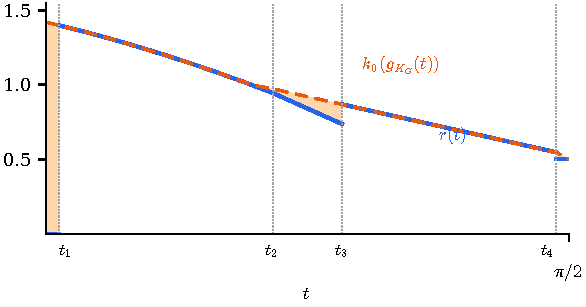
\includegraphics[width=0.78\linewidth]{figures/fig-curvature}
\caption{The first curvature bound for Gerver's cap, which maximizes $\cA$ (\cref{fact:optimal}): the density $r(t)$ of $\sigma_{\KG}$ on $[0,\pi/2)$ (blue) lies
below $k_0(g_{\KG}(t))$ (orange, dashed), computed from Romik's rotation path. They agree on $[t_1,t_*]$, where $g_{\KG}(t_*)=2$ ($t_*=0.616\ldots$), and on $[t_3,t_4]$; the gap is shaded.}
\label{fig:curvature}
\end{figure}

\subsection{The injectivity condition}

\begin{lemma}[integral inequalities]\label{lem:integral}
Let $K\in\Kc_{\pi/2}$ satisfy the curvature bounds. Then $K$ satisfies condition (1) of \cref{def:inj}, and
\begin{gather*}
  f_K(t)-1\ge\int_0^tm_0\bigl(g_K(u)\bigr)\dd u\quad(0\le t<\tfrac\pi2),\\
  g_K(t)-1\ge\int_t^{\pi/2}m_0\bigl(f_K(u)\bigr)\dd u\quad(0<t\le\tfrac\pi2).
\end{gather*}
\end{lemma}

\begin{proof}
Each restriction of $\sigma_K$ is dominated by a finite measure with a density, so it has a density
(Radon--Nikodym) and condition (1) holds. By \cref{fact:arms}\ref{fact:arms:regular}, $f_K,g_K$ are defined and continuous, $f_K(0)=1$, and
by \cref{fact:arms}\ref{fact:arms:integral}, for $t<\pi/2$,
$f_K(t)-1=\int_0^tg_K-\sigma_K((0,t])\ge\int_0^t(g_K-k_0(g_K))=\int_0^tm_0(g_K)$. For the second inequality apply the first to the
reflection $K^{\mir}$, which satisfies the curvature bounds with their roles exchanged, and use
\cref{fact:arms}\ref{fact:arms:mirror}: $f_{K^{\mir}}(s)=g_K(\pi/2-s)$ and $g_{K^{\mir}}(s)=f_K(\pi/2-s)$, with $t=\pi/2-s$.
\end{proof}

\begin{lemma}[the lower sequence]\label{lem:lower}
Let $f,g:[0,\pi/2]\to[0,\infty)$ be continuous with $f(t)-1\ge\int_0^tm_0(g)$ for $t\in[0,\pi/2)$ and
$g(t)-1\ge\int_t^{\pi/2}m_0(f)$ for $t\in(0,\pi/2]$. Then for every $j\ge0$, $f_j(t)\le f(t)$ on $[0,\pi/2)$ and
$f_j(\pi/2-t)\le g(t)$ on $(0,\pi/2]$.
\end{lemma}

\begin{proof}
Induction on $j$, the case $j=0$ being $f_0=0\le f,g$. If it holds for $j$, then for $t\in[0,\pi/2)$, since $m_0$ is
nondecreasing and $f_j(\pi/2-u)\le g(u)$ for $u\in(0,t]$,
$\mathcal Ff_j(t)=1+\int_0^tm_0(f_j(\pi/2-u))\dd u\le1+\int_0^tm_0(g)\le f(t)$, and with $f_j\le f$ we get
$f_{j+1}=\max(f_j,\mathcal Ff_j)\le f$ on $[0,\pi/2)$. For $t\in(0,\pi/2]$,
$\mathcal Ff_j(\pi/2-t)=1+\int_t^{\pi/2}m_0(f_j(s))\dd s\le1+\int_t^{\pi/2}m_0(f)\le g(t)$, and with
$f_j(\pi/2-t)\le g(t)$ this gives $f_{j+1}(\pi/2-t)\le g(t)$.
\end{proof}

\begin{proposition}[injectivity]\label{prop:inj}
Every $K\in\Kc_{\pi/2}$ that satisfies the curvature bounds satisfies the injectivity condition, and
$f_K,g_K>1$ on $(0,\pi/2)$.
\end{proposition}

\begin{proof}
By \cref{lem:integral}, $K$ satisfies (1) and the integral inequalities, and $f_K,g_K$ are continuous and nonnegative.
By \cref{lem:lower} and \cref{fact:iteration}\ref{fact:iteration:eleven}, for $t\in(0,\pi/2)$,
$1<f_{11}(t)\le f_K(t)$ and $1<f_{11}(\pi/2-t)\le g_K(t)$. By \cref{fact:arms}\ref{fact:arms:regular}, $\xx_K$ is continuously differentiable with
$\xx_K'=-(f_K-1)u_t+(g_K-1)v_t$, which gives (2) and (3).
\end{proof}

\begin{corollary}[maximizing right-angle caps are in $\Ki$]\label{cor:Ki}
Every $K\in\Kc_{\pi/2}$ with $\cA(K)=\abs\Gs$ lies in $\Ki$.
\end{corollary}

\begin{proof}
$K$ is maximizing (\cref{fact:optimal}) and $\cA(K)=\abs\Gs>0$, so it satisfies the curvature bounds
(\cref{prop:curvature}) and the injectivity condition (\cref{prop:inj}); and $\abs K\ge\cA(K)=\abs\Gs\ge11/5$.
\end{proof}
